\documentclass[final]{rapport1}
\usepackage[utf8]{inputenc}
\usepackage[export]{adjustbox} 
\usepackage{pdfpages}
\usepackage{graphicx}
\usepackage{authblk}
\usepackage[danish]{babel}
\usepackage{csquotes}
\usepackage[nottoc]{tocbibind}
\addto{\captionsdanish}{\renewcommand{\abstractname}{Abstract}}


\begin{document}
\begin{titlepage}
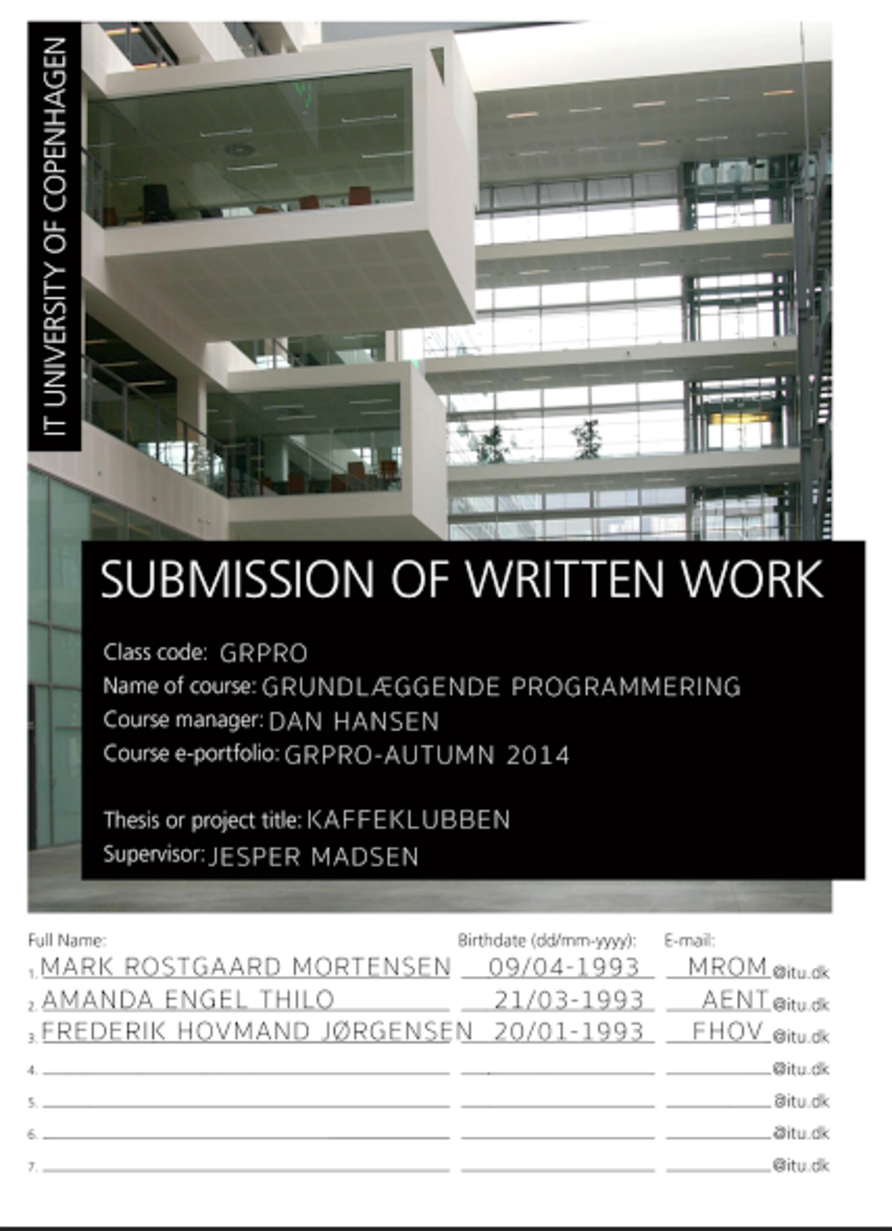
\includepdf{frontpage.pdf}
\end{titlepage}



\includepdf[width=400pt]{forside.pdf}



 
\baselineskip= 15pt

\begin{abstract}

In this report we address our workgroups attempt at designing a digital solution for broadening the audience for both the digital and physical offerings, that Statens Museum for Kunst(SMK) provides. We use a multitude of idea generation techniques, to arrive at a product, and then interviews with SMK. We propose an enhanced web-presence, for image viewing and discussion, based on feedback from SMK and visits to the museum. The report concludes with the proposal of a system in which users can comment and interact with the different artworks on the website.

\end{abstract}
\clearpage
\tableofcontents
\chapter{Forord}


\chapter{Indledning}
\section{Baggrund}
Det problemområde vi har arbejdet med i forbindelse med vores projekt, er udviklingen af et softwaresystem til brug for en ekspedient der betjener en billetluge i en biograf. Det område der skulle dækkes var reservation både når kunden stod foran billetlugen, samt når kunden ringede ind på telefon. Vores løsning skulle håndtere   ekspedientens arbejdsopgaver i sådanne situationer. Løsningen skal derfor fokusere udelukkende på reservationer, og ikke salg. 

\section{Problemstilling}
Den overordnede problemstilling som vores program besvarer, er hvordan man udviklinger et simpelt, brugervenligt og databasebaseret softwaresystem til brug for en ekspident i en billetluge. 

\subsection{Krav til programmet}
Af krav til porgrammet kan nævnes at der i forbindelse med reservationerne skal oplyses navn eller anden identitet på kunden. Vi har i vores program valgt at den centrale information omkring brugeren er dennes telefonnummer. Det har vi gjort af den grund af flere kunder godt kan have samme navn, men at ens telefonnummer er unikt.  

Derudover skal biografen indeholde flere sale, og sende flere forskellige forestillinger i løbet af dagen. Salenes størrelse, antal pladser mm. skal fremgå af databasen frem for at være indkodet i selve programteksten. Derfor har vi i stedet for at skrive data ind i programteksten, valgt at lave en speciel klasse til at hente data fra databasen. 

Det samme er gældende for de enkelte forestillinger, der derfor også bliver gemt i databasen.

\subsection{Brugerscenario} - skal laves om
Når ekspedienten åbner vores biobooking-system vil der på venstre side af vinduet være oplistet de film der spilles i biografen i øjeblikket. Klikker ekspedienten på en af disse film vil der på højre side af vinduet vise sig de tilhørende spilletider til den valgte film. Klikker ekspedienten derimod ikke på noget, vil der stå følgene tekst \emph{Klik på en film til venstre for at vise tidspunkter}. Øverst oppe i vinduet vil man se tre faner: \emph{Forestillinger, Reservation og Ret reservation}. Man kan godt navigere mellem fanerne, men har man ikke først valgt film og tidspunkt vil \emph{Reservation} være ubrugelige.
 
Efter at ekspedienten har valgt en film og en spilletid vil systemet automatisk skifte videre til den næste fane: \emph{Reservation}. Her kan ekspedienten vælge frit mellem de ledige sæder. Dette gøres ved at ekspedienten enten klikker enkeltvis på de grønne sæder, eller ved at trække musen over de ønskede sæder. De valgte sæder vil nu blive blå, så ekspedienten kan se hvilke der er valgt. Er sæderne tilfredsstillende skal ekspedienten skrive navn samt telefonnummer på kunden ind i et informationsfelt nedernst til højre på siden. Nedderst på siden ses i venstre hjørne antallet af sæder i alt, samt det ledige antal sæder. Dette kan ekspedienten også se på det grafiske billede over biografsalen, da de allerede reserverede sæder er røde, samt umulige at vælge for reservation. Efter kundens information er indtastet og ekspedienten har klikket på \emph{Fuldfør reservation} kommer et pop-up vindue op, hvor der står skrevet: \emph{Bestillingen er gennemført}.

Ønsker den pågældende kunde derimod at ændre eller slette en reservation, skal ekspedienten klikke sig ind på den sidste fane: \emph{Ret reservation}. På denne side finder ekspedienten øverst oppe et input felt hvor kundens telefonnumer skal indtastes. Når ekspedienten har klikket enter vil kundens reservation(er) dukke op nedenfor i en pæn liste. Ekspedienten kan så klikke på den reservation som kunden ønsker ændret. Nu føres ekspedienten til en popup \emph{Reservation} side, hvor de sæder tilknyttet den pågældende reservation nu ses med blåt. Ekspedienten kan således tilføje eller fjerne sæder ved at klikke på sæder med musen og derefter klikke på \emph{Ret reservation}. Ønsker kunden helt at slette reservationen kan dette lade sig gøre ved at klikke på \emph{Slet reservation}. 

\subsection{Systemdesign}
Vores system er overordnet baseret på data fra databasen. Systemet generer layout ud fra forskellige data i databasen. Dette indebærer bl.a. hvilke film der er i film-tabellen, hvilke forestillinger der er tilknyttet til en given film, hvilke reservationer der er tilknyttet en given forestilling, hvilke reservationer der er tilknyttet et givent telefonnummer mv. Programmet er delt op, så mest mulig databehandling foretages hos klienten/brugeren. Dette indebærer objekter med informationer om de forskellige forestillinger, arrays med valgte sæder mv. Databaseforespørgsler er lavet så omfattende som muligt, så der udføres så få forespørgsler som muligt og data gemmes i objekter og arrays eller bliver benyttet med det samme i den grafiske fremstilling af programmet som eksempelvis ved generering af film-knapper. 


\chapter{Problemanalyse}
\section{Vores løsning}
Den overordnede problemstilling som vi har valgt at fokusere på at løse er hvordan man udvikler et simpelt og implecit program som er brugervenligt og med så lidt data som muligt i selve programkoden.


Vores program løser problemstilligen ved at have alt information omkring forestillinger, sale, film og reservationer gemt i en database. Dette gør selve programteksen simpel og nem at ændre i, og vi har på den måde undgået for meget kodeduplikering. For at opfylde ønsket om brugervenlighed har vi valgt at vise størstedelen af programmet i ét vindue, hvor brugeren så nemt kan navigere mellem de forskellige muligheder programmet har. 


\subsection{Alternative løsninger}
An alternativ måde at løse problemstillingen på ville være at fokusere på andre måder at booke billetter på. Vi har valgt at man først skal vælge film, derefter tid og sæder. Man kunne have valgt at gøre det muligt for brugeren at vælge data eller tid før valg af film. Vi har blot valgt den løsning vi syntes var mest brugervenlig. En anden mulighed er at man kunne have lavet en liste der viste \emph{alle} forestillinger sorteret efter spilletid - uden at tage hensyn til sortering i forhold til film. Denne mulighed syntes vi designmæssigt ville fungere meget rodet. Derudover kunne vi have valgt at gemme vores reservationer i programkoden frem for i databasen. Vi diskuterede dette i begyndelsen af projektet, men fandt det for besværligt at arbejde med, da det ville kræve støre mængder kode, fylde mere plads samt resultere i at vores program formentlig ville brugere længere tid på at compille og kører. 

\section{Databasedesign}
En af de to overordnede tabeller i vores database er \emph{cinemas} som indeholder information omkring vores biografsale. Dette omfatter salens navn, id, antal rækker og antal sæder i hver række. Vores sæder er ikke repræsenteret som en tabel i vores database, men derimod gemt som et 2 dimentionelt array. 

Den anden vigtige tabel er \emph{movies} som indeholder inforamtion omkring de film der går i biografen. Det eneste inforamtion denne tabel holder er navn og id.

I begge tabel er det, det pågældende id som fungerer som nøgle. Altså sal\_id og movie\_id.  

De to tabeller \emph{movie} og \emph{cinema} bliver koblet sammen i tabellen \emph{show}. Her bruges deres nøgler til at sammensætte de foreskellige forestillinger som vores biograf kan vise. I \emph{shows} tilføjes så et nyt ide til de enkelte forestillinger samt et timestamp - som er det tidspunkt forestillingen skal begynde.


\chapter{Brugervejledning}
\section{Programmet}
Programmet er designet med 3 tabs i toppen. \emph{Forestillinger, Reservation og Ret reservation}. Når programmet åbnes starter brugeren i \emph{Forestillinger-vinduet} og der vises en liste i venstre side med de film som kører i biografen. Brugeren klikker på den film, som kunden ønsker at reservere billetter til. Når en film vælges bliver tiderne for filmforestillinger vist for den pågældende film. \\


\begin{picture}

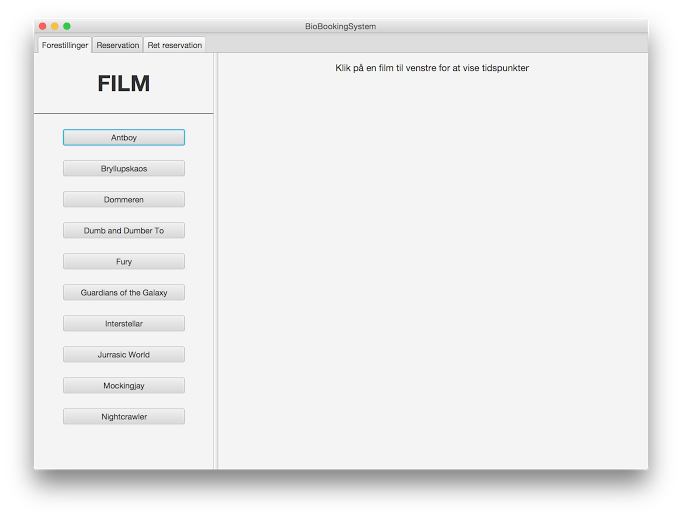
\includegraphics[width=150pt]{1.png}
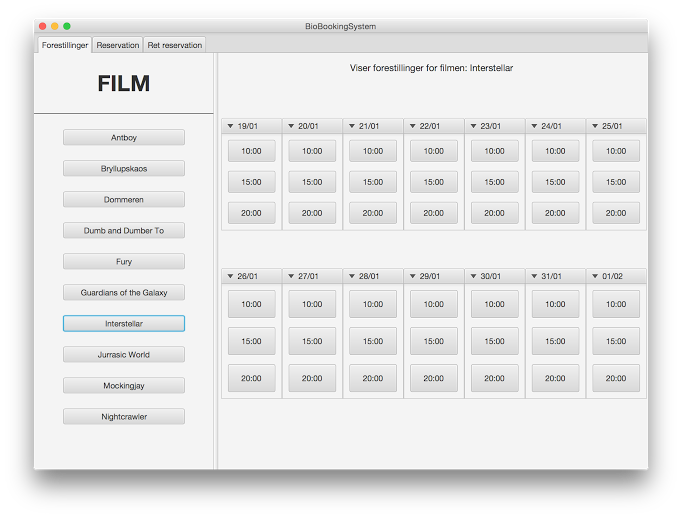
\includegraphics[width=150pt]{2.png}

\end{picture}
\begin{center}
\tiny Figure 1. Forestillinger-vinduet før og efter en film er valgt
\end{center}

Klikker ekspedienten derimod ikke på noget, vil der stå følgene tekst \emph{Klik på en film til venstre for at vise tidspunkter}, og har man ikke først valgt film og tidspunkt vil \emph{Reservation} være ubrugelige.

Efter at have valgt film, vælger brugeren tidspunktet, som kunden ønsker at reservere til. Når en forestilling vælges bliver brugeren videreført til næste tab - altså reservation. Her vises et vindue med firkanter som illustrerer sæderne i biografen. Ledige sæder er illustreret som en grøn firkant og optagede sæder er illustreret som røde sæder. Brugeren klikker på de sæder som kunden ønsker at reservere - brugeren kan desuden holde musen nede og hive musen over de sæder som skal vælges. De valgte sæder skifter farve til blå og brugeren kan se hvor mange sæder vedkommende har markeret nederst i venstre hjørne. 

\begin{picture}

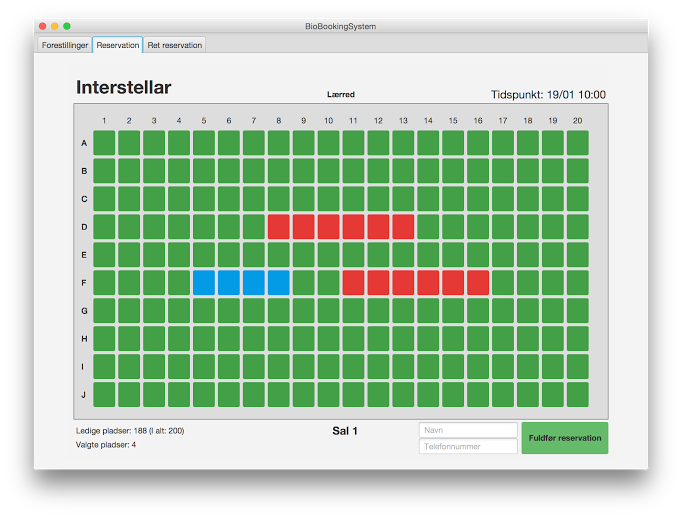
\includegraphics[width=250pt]{3.png}

\end{picture}
\begin{center}
\tiny Figure 2. Biograf sal med reserverede sæder i rødt, samt sæder brugeren er ved at reservere i blå
\end{center}

Når sæderne er valgt skrives kundens navn og telefonnummer ind i tekstfelterne nederst i højre hjørne. Afslutningsvist trykkes der på knappen \emph{Fuldfør reservation}. 

<<<<<<< HEAD
Hvis kunden fortryder sin bestilling eller har ændringer til en eksisterende bestilling, så klikker brugeren på tabben \emph{Ret reservation} i toppen af programmet. Brugeren bliver taget til et vindue hvor kundens telefonnummer skal indtastes. Når telefonnummeret er indtastet og der er trykket på Enter-tasten eller på \emph{Tjek reservationer}-knappen, så vises en liste nedenunder med de reservationer som kunden har tilknyttet til sit telefonnummer. Der vises kun reservationer for forestillinger som ikke er blevet vist - gamle reservationer vises altså ikke. Brugeren dobbeltklikker på den reservation der skal rettes og et nyt vindue åbner som ligner reservationsvinduet. De optagede sæder er røde, de ledige er grønne og de sæder som er tilknyttet til den pågældende reservation vises som blå. Brugeren kan tilføje eller slette sæder. Et valgt er blåt og markeringen fjernes ved at klikke på sædet igen. Når ændringen til reservationen er valgt, så klikker brugeren på \emph{Rediger reservation}. Skal reservationen derimod slettes helt, så klikker brugeren på \emph{Slet reservation}.styffff
=======
Hvis kunden fortryder sin bestilling eller har ændringer til en eksisterende bestilling, så klikker brugeren på tabben \emph{Ret reservation} i toppen af programmet. Brugeren bliver taget til et vindue hvor kundens telefonnummer skal indtastes. Når telefonnummeret er indtastet og der er trykket på Enter-tasten eller på \emph{Tjek reservationer}-knappen, så vises en liste nedenunder med de reservationer som kunden har tilknyttet til sit telefonnummer. \\
>>>>>>> ef25a562ca38edd3c851bfc283f11a238cb2f839

\begin{picture}

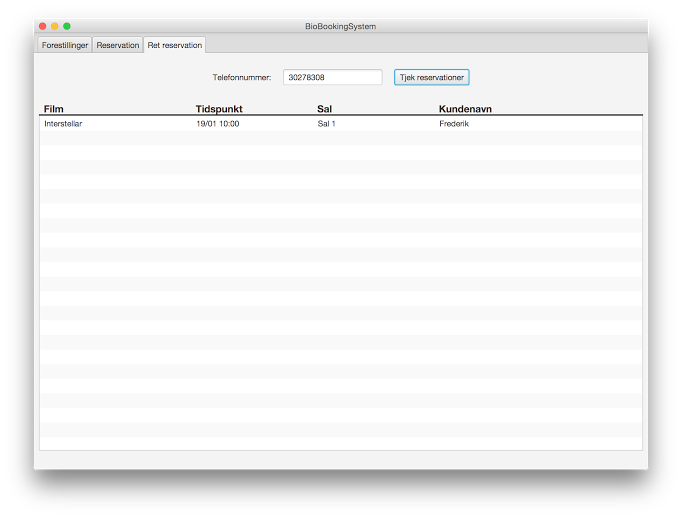
\includegraphics[width=250pt]{4.png}

\end{picture}
\begin{center}
\tiny Figure 3. Forestillinger-vinduet før og efter en film er valgt
\end{center}

Der vises kun reservationer for forestillinger som ikke er blevet vist - gamle reservationer vises altså ikke. Brugeren dobbeltklikker på den reservation der skal rettes og et nyt vindue åbner som ligner reservationsvinduet. \\

\begin{picture}

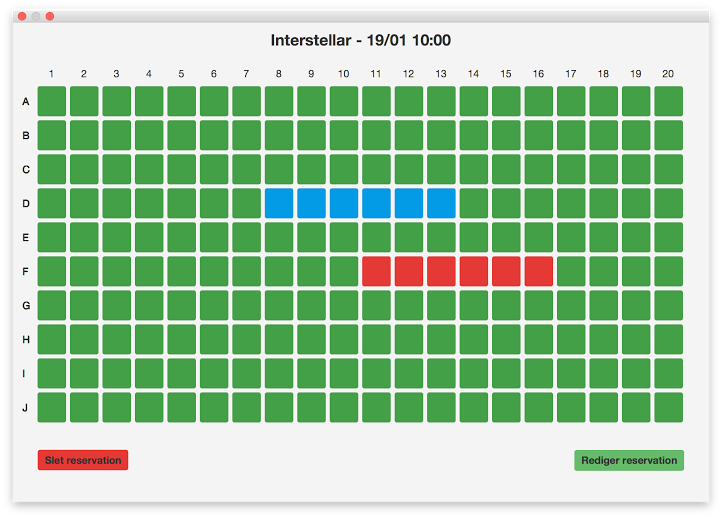
\includegraphics[width=250pt]{5.png}

\end{picture}
\begin{center}
\tiny Figure 4. Vinduet hvor brugeren retter sin reservation
\end{center}

De optagede sæder er røde, de ledige er grønne og de sæder som er tilknyttet til den pågældende reservation vises som blå. Brugeren kan tilføje eller slette sæder. Et valgt er blåt og markeringen fjernes ved at klikke på sædet igen. Når ændringen til reservationen er valgt, så klikker brugeren på \emph{Rediger reservation}. Skal reservationen derimod slettes helt, så klikker brugeren på \emph{Slet reservation}.

\subsection{Begrænsninger}
\subsection{Fejlmeddelelser}
\section{Eksempel}

\chapter{Teknisk Analyse}
\section{Model View Controller}

\subsection{Moduler}
Programmet har 2 klasser: DBConnect og buildHolder.
DBConnect foretager alt der har med databasen at gøre. Dette er eksempelvis databaseforespørgsler hvor alle film returneres i et LinkedHashMap, hvor data såsom reservationer, salstørrelse mv. for en given forestilling hentes, hvor data såsom reservationer indsættes eller opdateres i databasen. Den væsentligste del af DBConnect-klassen må være funktionen getCon, der sørger for at der er en gyldig forbindelse til databasen. 
buildHolder er et objekt hvor data for en given forestilling lagres. Der bruges getters og setters, så de data der lagres også kan hentes efterfølgende. buildHolder objektet bruges efterfølgende til at bygge reservationssalen med data som filmnavn, tidspunkt for forestillingen, størrelsen på salen (rows/columns), reserverede sæder mv. 

Det er controlleren der gør brug af disse objekter, når data skal visualiseres og altså fremvises for brugeren.

\subsection{Datastrukturer}

\subsection{Algoritmer}

\section{Brugergrænsedesign}

%\begin{itemize}
%\item 
%\item 
%\item 
%\item 
%\item 
%\end{itemize}



\subsection{Begrænsninger}

\chapter{Afprøvning}

\section{Brugerafprøvning}

\section{Unitet}

\section{Afprøvnings konklusion}


\chapter{Konklusion}

\chapter{Litteratur}

\chapter{Bilag}

\end{document}






